\documentclass[12pt]{article}
\usepackage{amsmath}
\usepackage{amssymb}
\usepackage{graphicx}
\usepackage{subcaption}
\usepackage{cite}
\usepackage{hyperref}
\usepackage{float}

\title{Path Tracing Renderer Using Monte Carlo Methods}
\author{Silas Maughan}
\date{\today}

\begin{document}

\maketitle

\begin{abstract}
    This report presents a study on the implementation of a path tracing renderer using Monte Carlo methods to simulate realistic lighting in a 3D scene. Various sampling techniques and variance reduction methods are explored to enhance image quality and convergence speed. Experimental results demonstrate the effectiveness of these techniques in reducing noise and improving rendering efficiency. The report discusses the mathematical foundations, implementation details, and performance evaluations of different Monte Carlo sampling strategies and variance reduction techniques.
\end{abstract}

\tableofcontents

\section{Introduction}
\label{sec:intro}
\subsection{Purpose and Scope}
\subsubsection{Goals of the Document}
The goal of this document is to explain the implementation of a path tracing renderer using Monte Carlo methods, focusing on different sampling techniques and variance reduction methods to enhance image quality and rendering efficiency.
\subsubsection{Overview of the Methodological Approach}
The methodological approach will be outlined and the effectiveness of these techniques will be evaluated through experimental results.

\subsection{Background}
\subsubsection{Overview of Ray Tracing}
Path tracing is a rendering technique used to create realistic images by simulating the way light interacts with objects in a scene. Unlike traditional ray tracing, which traces a single path of light from the eye to the light source, path tracing traces multiple light paths to account for complex interactions like reflection, refraction, and scattering. This report details the implementation of a path tracing renderer using Monte Carlo integration to approximate the rendering equation.
\subsubsection{Importance in Computer Graphics}
Path tracing is crucial in computer graphics for achieving photo-realistic rendering, as it accurately simulates the physical behavior of light.

\section{Ray Tracing Fundamentals}
\label{sec:fundamentals}

\subsection{Rays}
\subsubsection{Definition of a Ray}
A ray in 3D graphics is an essential construct for simulating the propagation of light through a scene. It is defined by an origin point \(\mathbf{O}\) and a direction vector \(\mathbf{D}\). Mathematically, we can express a point \(\mathbf{P}(t)\) along the ray as:
\[
    \mathbf{P}(t) = \mathbf{O} + t\mathbf{D}
\]
where \(t\) is a real number parameter. This equation indicates that the ray starts at the origin \(\mathbf{O}\) and extends infinitely in the direction of \(\mathbf{D}\). In practical terms, \(t\) is typically constrained within an interval \([t_{\text{min}}, t_{\text{max}}]\) to define a segment of the ray.

The geometric interpretation of a ray is straightforward: it represents a half-line extending from \(\mathbf{O}\). This formulation is crucial for tracing the path of light as it interacts with objects in a scene.

\subsubsection{Ray-Object Intersection}
At the core of ray tracing is the need to determine whether a ray intersects an object in the scene. This involves solving for \(t\) when a point \(\mathbf{P}(t)\) on the ray lies on the surface of the object. Each type of object requires a specific intersection test, leading to a variety of mathematical formulations.

\subsection{Vectors and Their Operations}
Vectors play a pivotal role in ray tracing, representing points, directions, normals, and colors. A 3D vector \(\mathbf{A}\) can be represented as \((A_x, A_y, A_z)\). We will cover essential vector operations that are fundamental to ray tracing.

\subsubsection{Dot Product}
The dot product of two vectors \(\mathbf{A}\) and \(\mathbf{B}\) is a scalar quantity given by:
\[
    \mathbf{A} \cdot \mathbf{B} = A_x B_x + A_y B_y + A_z B_z
\]
The dot product is used to calculate the angle between two vectors, determine orthogonality, and compute projections. For example, the angle \(\theta\) between \(\mathbf{A}\) and \(\mathbf{B}\) can be found using:
\[
    \cos(\theta) = \frac{\mathbf{A} \cdot \mathbf{B}}{\|\mathbf{A}\| \|\mathbf{B}\|}
\]

\subsubsection{Cross Product}
The cross product of two vectors \(\mathbf{A}\) and \(\mathbf{B}\) results in a third vector \(\mathbf{C}\) that is perpendicular to both:
\[
    \mathbf{C} = \mathbf{A} \times \mathbf{B} = \left( A_y B_z - A_z B_y, A_z B_x - A_x B_z, A_x B_y - A_y B_x \right)
\]
The magnitude of \(\mathbf{C}\) is given by:
\[
    \|\mathbf{C}\| = \|\mathbf{A}\| \|\mathbf{B}\| \sin(\theta)
\]
where \(\theta\) is the angle between \(\mathbf{A}\) and \(\mathbf{B}\).

\subsection{Intersection Calculations}
\subsubsection{Spheres}
A sphere is a common geometric object in ray tracing, defined by its center \(\mathbf{C}\) and radius \(R\). To determine the intersection of a ray with a sphere, we substitute the ray equation \(\mathbf{P}(t) = \mathbf{O} + t\mathbf{D}\) into the sphere's implicit equation:
\[
    \left\| \mathbf{P}(t) - \mathbf{C} \right\|^2 = R^2
\]
Expanding and simplifying this equation yields:
\[
    \left\| \mathbf{O} + t\mathbf{D} - \mathbf{C} \right\|^2 = R^2
\]
\[
    \left( \mathbf{O} - \mathbf{C} + t\mathbf{D} \right) \cdot \left( \mathbf{O} - \mathbf{C} + t\mathbf{D} \right) = R^2
\]
\[
    (\mathbf{O} - \mathbf{C}) \cdot (\mathbf{O} - \mathbf{C}) + 2t \left( \mathbf{O} - \mathbf{C} \right) \cdot \mathbf{D} + t^2 \mathbf{D} \cdot \mathbf{D} = R^2
\]
This is a quadratic equation in \(t\):
\[
    t^2 \mathbf{D} \cdot \mathbf{D} + 2t \left( \mathbf{O} - \mathbf{C} \right) \cdot \mathbf{D} + \left( (\mathbf{O} - \mathbf{C}) \cdot (\mathbf{O} - \mathbf{C}) - R^2 \right) = 0
\]
Letting \(\mathbf{L} = \mathbf{O} - \mathbf{C}\), \(a = \mathbf{D} \cdot \mathbf{D}\), \(b = 2 \mathbf{L} \cdot \mathbf{D}\), and \(c = \mathbf{L} \cdot \mathbf{L} - R^2\), we solve the quadratic equation:
\[
    at^2 + bt + c = 0
\]
The solutions for \(t\) are given by:
\[
    t = \frac{-b \pm \sqrt{b^2 - 4ac}}{2a}
\]
The discriminant \(b^2 - 4ac\) determines the nature of the intersection:
\begin{itemize}
    \item If \(b^2 - 4ac < 0\), the ray does not intersect the sphere.
    \item If \(b^2 - 4ac = 0\), the ray tangentially intersects the sphere at one point.
    \item If \(b^2 - 4ac > 0\), the ray intersects the sphere at two points.
\end{itemize}

\subsubsection{Planes}
A plane is defined by a point \(\mathbf{P}_0\) on the plane and a normal vector \(\mathbf{N}\). To find the intersection of a ray with a plane, we use the plane equation:
\[
    \mathbf{N} \cdot \left( \mathbf{P}(t) - \mathbf{P}_0 \right) = 0
\]
Substituting the ray equation \(\mathbf{P}(t) = \mathbf{O} + t\mathbf{D}\):
\[
    \mathbf{N} \cdot \left( \mathbf{O} + t\mathbf{D} - \mathbf{P}_0 \right) = 0
\]
\[
    \mathbf{N} \cdot \mathbf{O} + t \left( \mathbf{N} \cdot \mathbf{D} \right) - \mathbf{N} \cdot \mathbf{P}_0 = 0
\]
Solving for \(t\):
\[
    t = \frac{\mathbf{N} \cdot (\mathbf{P}_0 - \mathbf{O})}{\mathbf{N} \cdot \mathbf{D}}
\]
provided \(\mathbf{N} \cdot \mathbf{D} \neq 0\). If \(\mathbf{N} \cdot \mathbf{D} = 0\), the ray is parallel to the plane and does not intersect it.

\subsection{Color and Shading Models}
\subsubsection{Light and Material Interaction}
The appearance of objects in a scene is influenced by how they interact with light. When light strikes a surface, it can be absorbed, reflected, or transmitted. These interactions are governed by the material properties of the surface.

\subsubsection{Diffuse Reflection}
A perfectly diffuse (Lambertian) surface scatters incident light uniformly in all directions. The intensity \(I\) of the reflected light is proportional to the cosine of the angle \(\theta\) between the light direction \(\mathbf{L}\) and the surface normal \(\mathbf{N}\):
\[
    I = I_0 \cdot \max(\mathbf{L} \cdot \mathbf{N}, 0)
\]
where \(I_0\) is the intensity of the incoming light. This cosine dependency ensures that light hitting the surface at a shallow angle contributes less to the reflected intensity.

\subsubsection{Specular Reflection}
Specular reflection occurs on shiny surfaces where light is reflected in a specific direction. The reflection vector \(\mathbf{R}\) is computed as:
\[
    \mathbf{R} = \mathbf{L} - 2(\mathbf{L} \cdot \mathbf{N})\mathbf{N}
\]
The intensity of the reflected light depends on the angle between the reflection vector \(\mathbf{R}\) and the view direction \(\mathbf{V}\):
\[
    I = I_0 \cdot \max(\mathbf{V} \cdot \mathbf{R}, 0)^n
\]
where \(n\) is the shininess coefficient, determining the sharpness of the reflection.

\subsubsection{Technical Implementation}
Color models in code often represent colors as vectors with three components: red, green, and blue (RGB). Each component ranges from 0 to 1.

*Lambertian Reflectance:* In a Lambertian model, the scattering of rays is uniformly distributed over the hemisphere centered on the surface normal. This can be implemented using Monte Carlo techniques to randomly sample directions within the hemisphere.

\begin{figure}[H]
    \centering
    \begin{subfigure}[b]{0.45\textwidth}
        \centering
        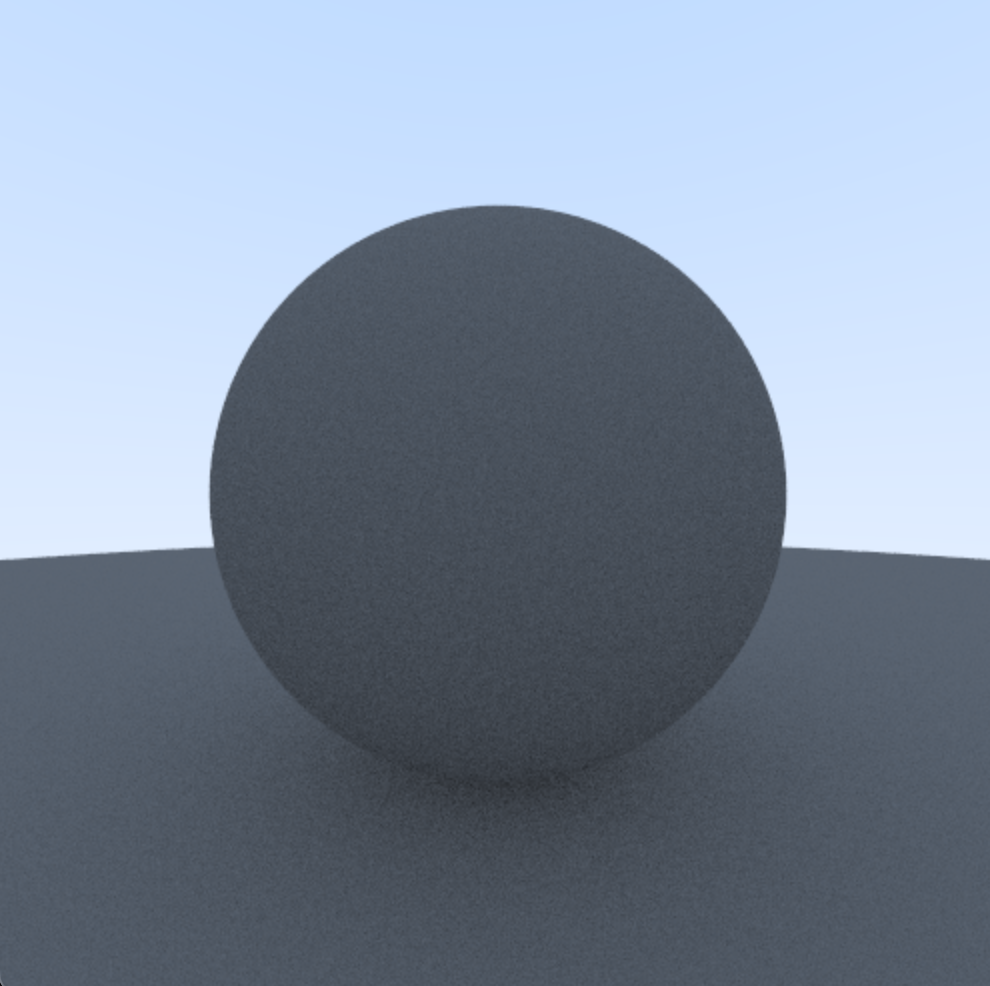
\includegraphics[width=\textwidth]{images/uniform_diffuse.png}
        \caption{Rendered image using Uniform Diffuse Renderer}
        \label{fig:completely_diffuse}
    \end{subfigure}
    \hfill
    \begin{subfigure}[b]{0.45\textwidth}
        \centering
        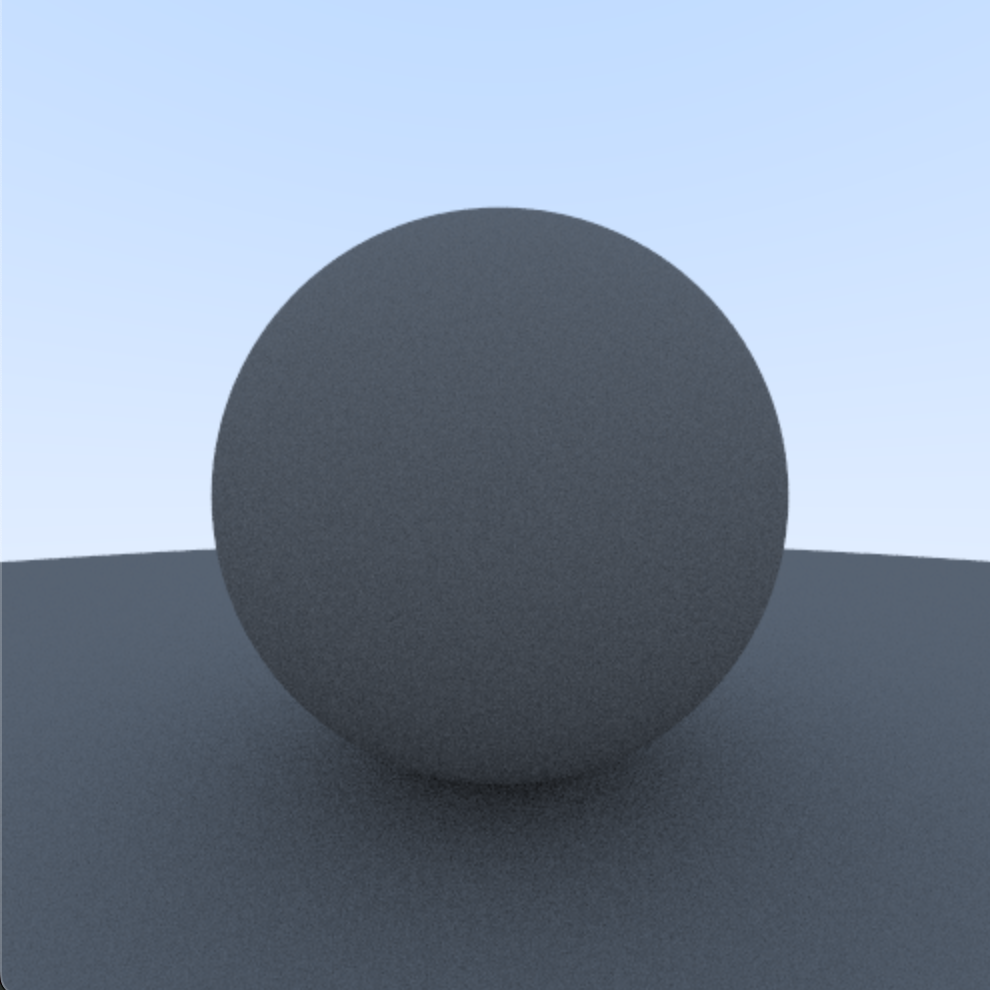
\includegraphics[width=\textwidth]{images/lambertian_diffuse.png}
        \caption{Rendered image using Lambertian Diffuse Renderer}
        \label{fig:lambertian_diffuse}
    \end{subfigure}
    \caption{Comparison of rendering techniques}
    \label{fig:rendering_comparison}
\end{figure}

*Specular Reflectance:* For specular materials, the direction of the reflected ray is computed using the reflection equation. This is crucial for simulating shiny surfaces such as metals and mirrors.

\subsection{Linear Transformations}
\subsubsection{Translation, Rotation, and Scaling}
Objects in a 3D scene can be manipulated using transformations such as translation, rotation, and scaling. These transformations are represented by matrices.

*Translation:* A translation matrix \(\mathbf{T}\) moves an object by a vector \(\mathbf{d} = (d_x, d_y, d_z)\):
\[
    \mathbf{T} = \begin{pmatrix}
        1 & 0 & 0 & d_x \\
        0 & 1 & 0 & d_y \\
        0 & 0 & 1 & d_z \\
        0 & 0 & 0 & 1
    \end{pmatrix}
\]

*Rotation:* A rotation matrix \(\mathbf{R}\) rotates an object around an axis. For example, a rotation around the \(z\)-axis by an angle \(\theta\) is given by:
\[
    \mathbf{R}_z(\theta) = \begin{pmatrix}
        \cos \theta & -\sin \theta & 0 & 0 \\
        \sin \theta & \cos \theta  & 0 & 0 \\
        0           & 0            & 1 & 0 \\
        0           & 0            & 0 & 1
    \end{pmatrix}
\]

*Scaling:* A scaling matrix \(\mathbf{S}\) scales an object by factors \(s_x\), \(s_y\), and \(s_z\):
\[
    \mathbf{S} = \begin{pmatrix}
        s_x & 0   & 0   & 0 \\
        0   & s_y & 0   & 0 \\
        0   & 0   & s_z & 0 \\
        0   & 0   & 0   & 1
    \end{pmatrix}
\]

\subsubsection{Matrix Representations}
Transformation matrices allow for the linear transformation of vectors. Given a vector \(\mathbf{v}\) and a transformation matrix \(\mathbf{M}\), the transformed vector \(\mathbf{v}'\) is:
\[
    \mathbf{v}' = \mathbf{M} \mathbf{v}
\]
Combining multiple transformations is achieved by matrix multiplication.

\subsubsection{Technical Implementation}
*Transforming Objects and Rays:* Applying matrix operations to objects and rays in the scene ensures consistent transformations. The composite matrix \(\mathbf{M}\) for a series of transformations is:
\[
    \mathbf{M} = \mathbf{T} \mathbf{R} \mathbf{S}
\]

*Applying Transformations to the Scene:* All elements in the scene, including geometry and light sources, are transformed using composite matrices to maintain spatial coherence.




\section{Advanced Techniques in Ray Tracing}
\label{sec:advanced}

\subsection{Camera and Viewing}
\label{subsec:camera-viewing}

\subsubsection{Camera Model and Rays}
The camera in ray tracing simulates the viewpoint from which the scene is rendered. It projects rays from its origin through each pixel on the image plane, capturing the scene from a specific perspective. The mathematical foundation underlying the camera's functionality involves various concepts from linear algebra.

\paragraph{Basis Vectors and Camera Orientation}

\subparagraph{Basis Vectors}
The camera's orientation is defined by three orthonormal basis vectors: \(\mathbf{u}\), \(\mathbf{v}\), and \(\mathbf{w}\).
\begin{itemize}
    \item \(\mathbf{w}\): Vector pointing from the camera position to the view direction. It is computed as:
          \[
              \mathbf{w} = \frac{\mathbf{C} - \mathbf{L}}{\|\mathbf{C} - \mathbf{L}\|}
          \]
          where \(\mathbf{C}\) is the camera position and \(\mathbf{L}\) is the focal point.
    \item \(\mathbf{u}\): Vector pointing to the right of the camera, computed using the cross product of the up vector \(\mathbf{v}_{\text{up}}\) and \(\mathbf{w}\):
          \[
              \mathbf{u} = \frac{\mathbf{v}_{\text{up}} \times \mathbf{w}}{\|\mathbf{v}_{\text{up}} \times \mathbf{w}\|}
          \]
    \item \(\mathbf{v}\): Vector pointing upwards relative to the camera, computed as:
          \[
              \mathbf{v} = \mathbf{w} \times \mathbf{u}
          \]
\end{itemize}

These basis vectors form a right-handed coordinate system and define the camera's orientation.

\paragraph{Viewport and Field of View}
The camera's field of view (FOV) determines the extent of the observable world. The vertical FOV (\(\text{vertFov}\)) is the angle of the observable world in the vertical direction:
\[
    \text{viewportHeight} = 2 \cdot \tan\left(\frac{\text{vertFov}}{2}\right)
\]
The viewport width is adjusted according to the aspect ratio (\(\text{aspectRatio}\)):
\[
    \text{viewportWidth} = \text{aspectRatio} \cdot \text{viewportHeight}
\]

\paragraph{Perspective Projection}
To generate rays from the camera through each pixel, we calculate the position of each pixel in the camera's coordinate system. The pixel positions are offset from a reference point (the upper-left corner of the viewport) by the basis vectors \(\mathbf{u}\) and \(\mathbf{v}\).

\paragraph{Implementation in Camera Class}
The `Camera` class encapsulates the logic for positioning and orienting the camera, as well as generating rays through the pixels.

\begin{verbatim}
class Camera
{
public:
    Camera(unsigned int imageWidth, unsigned int imageHeight, const glm::vec3 &pos, const glm::vec3 &focalPoint, const glm::vec3 &up, float vertFov, unsigned int samplesPerPixel, unsigned int maxDepth);
    Camera(unsigned int imageWidth, unsigned int imageHeight, const CamPos &camPos, unsigned int samplesPerPixel, unsigned int maxDepth);

    void render(const HittableList &world, std::vector<glm::vec3> &accumulationBuffer, std::vector<int> &sampleCount);

    int image_width;
    int image_height;

private:
    glm::vec3 center;
    glm::vec3 look_at;
    glm::vec3 vup;
    float vert_fov;
    int sample_per_pixel_per_frame;
    int sqrt_sample_per_pixel_per_frame;
    float recip_sqrt_sppf;
    int max_depth;

    glm::vec3 pixel00_loc;
    glm::vec3 pixel_delta_u;
    glm::vec3 pixel_delta_v;
    glm::vec3 u;
    glm::vec3 v;
    glm::vec3 w;

    void initialize();
    Ray getRandomRay(int x, int y) const;
    Ray getRandomStratifiedRay(glm::vec3 pixelCenter, int gridX, int gridY) const;
    glm::vec3 rayColor(const Ray &r, const HittableList &world, int depth) const;
};
\end{verbatim}

The `Camera` class includes member variables to store the camera's position, orientation, and configuration parameters.

\paragraph{Initialization and Basis Vector Calculation}
The `initialize` method sets up the camera's coordinate system using the basis vectors:

\begin{verbatim}
void Camera::initialize() {
    float theta = glm::radians(vert_fov);
    float h = tan(theta / 2);
    float viewport_height = 2.0f * h;
    float viewport_width = viewport_height * float(image_width) / float(image_height);

    w = glm::normalize(center - look_at);
    u = glm::normalize(glm::cross(vup, w));
    v = glm::cross(w, u);

    pixel00_loc = center - (u * viewport_width / 2.0f) - (v * viewport_height / 2.0f) - w;
    pixel_delta_u = u * viewport_width / float(image_width);
    pixel_delta_v = v * viewport_height / float(image_height);
}
\end{verbatim}

Here,
\begin{itemize}
    \item \(\mathbf{w}\) is calculated as the normalized vector from the camera position to the look-at point.
    \item \(\mathbf{u}\) is the normalized cross product of the up vector and \(\mathbf{w}\).
    \item \(\mathbf{v}\) is the cross product of \(\mathbf{w}\) and \(\mathbf{u}\).
\end{itemize}

\paragraph{Ray Generation}
The method `getRandomRay` generates rays from the camera through each pixel, considering anti-aliasing by randomly offsetting the ray within the pixel:

\begin{verbatim}
Ray Camera::getRandomRay(int x, int y) const {
    float u_offset = (x + random_float()) * recip_sqrt_sppf;
    float v_offset = (y + random_float()) * recip_sqrt_sppf;
    glm::vec3 ray_origin = center;
    glm::vec3 ray_direction = glm::normalize(pixel00_loc + u_offset * pixel_delta_u + v_offset * pixel_delta_v - center);
    return Ray(ray_origin, ray_direction);
}
\end{verbatim}

This method uses the basis vectors to compute the direction of the rays passing through each pixel, incorporating random offsets to achieve anti-aliasing.

\paragraph{Rendering}
The `render` method generates rays for each pixel and computes the color by tracing these rays through the scene. The final image is accumulated and averaged over multiple samples for anti-aliasing.

\begin{verbatim}
void Camera::render(const HittableList &world, std::vector<glm::vec3> &accumulationBuffer, std::vector<int> &sampleCount) {
    for (int y = 0; y < image_height; ++y) {
        for (int x = 0; x < image_width; ++x) {
            glm::vec3 color(0.0f);
            for (int s = 0; s < sample_per_pixel_per_frame; ++s) {
                Ray r = getRandomRay(x, y);
                color += rayColor(r, world, max_depth);
            }
            accumulationBuffer[y * image_width + x] += color;
            sampleCount[y * image_width + x] += sample_per_pixel_per_frame;
            glm::vec3 averagedColor = accumulationBuffer[y * image_width + x] / float(sampleCount[y * image_width + x]);
            // Store averagedColor in the image buffer
        }
    }
}
\end{verbatim}

This process ensures that each pixel's color is the result of multiple samples, reducing aliasing and producing a smoother image.

\paragraph{Geometric Interpretation and Linear Transformations}

\subparagraph{Changing Basis}
The camera's view can be thought of as a change of basis. The world coordinates are transformed into the camera's coordinate system defined by the basis vectors \(\mathbf{u}\), \(\mathbf{v}\), and \(\mathbf{w}\).

\subparagraph{Linear Transformations}
Linear transformations, represented by matrices, are used to position and orient the camera. The transformation from world coordinates to camera coordinates involves translating the camera to the origin and rotating the basis vectors to align with the standard axes.

\subparagraph{Concept of Vector Space}
The camera’s coordinate system forms a vector space where the basis vectors \(\mathbf{u}\), \(\mathbf{v}\), and \(\mathbf{w}\) span the space. The transformations applied to these vectors ensure linear independence, meaning they form a valid coordinate system for the camera.

\subparagraph{Systems of Linear Equations}
In rendering, solving systems of linear equations can be used to determine intersections of rays with objects, transformations, and more. These systems can be represented and solved using matrix methods and vector operations.

In conclusion, the `Camera` class in ray tracing leverages concepts from linear algebra such as basis vectors, linear transformations, and vector spaces to simulate the projection of rays through an image plane. This allows for accurate positioning, orientation, and rendering of the scene from the camera's perspective.
\subsection{Acceleration Structures}
\subsubsection{Bounding Volume Hierarchies (BVH)}
An advanced structure for efficient intersection tests.
\subsubsection{Technical Implementation}
\begin{itemize}
    \item \textbf{Efficient Ray-Object Intersection Tests:} Using BVH for faster intersection calculations.
    \item \textbf{Building and Traversing BVH:} Methods for constructing and navigating BVH structures.
\end{itemize}

\subsection{Anti-Aliasing and Sampling}
\subsubsection{Aliasing Problems in Rendering}
Understanding the impact of aliasing and methods to mitigate it.
\subsubsection{Supersampling and Adaptive Sampling}
Techniques to enhance image quality.
\subsubsection{Technical Implementation}
\begin{itemize}
    \item \textbf{Implementing Supersampling:} Methods for applying supersampling in rendering.
\end{itemize}

\section{Mathematical Methods for Ray Tracing}
\label{sec:math-methods}
\subsection{Probability and Monte Carlo Methods}
\subsubsection{Random Sampling Techniques}
Utilizing stochastic methods to improve sampling efficiency.
\subsubsection{Basic Probability Concepts}
Foundational principles applicable to Monte Carlo methods.
\subsubsection{Monte Carlo Integration}
Using random sampling to approximate integrals.
\subsubsection{Technical Implementation}
\begin{itemize}
    \item \textbf{Path Tracing:} Implementing Monte Carlo techniques in path tracing.
    \item \textbf{Importance Sampling and Russian Roulette:} Advanced Monte Carlo techniques to enhance efficiency.
\end{itemize}

\subsection{Integration for Lighting Models}
\subsubsection{Radiance and Light Transport Equations}
Mathematical models for light behavior.
\subsubsection{Numerical Integration Techniques}
Applying numerical methods to solve lighting equations.
\subsubsection{Technical Implementation}
\begin{itemize}
    \item \textbf{Implementing Global Illumination:} Techniques for comprehensive lighting calculations.
    \item \textbf{Integrating Direct and Indirect Lighting:} Methods to account for all lighting contributions.
\end{itemize}

\section{Technical Description of the System}
\label{sec:system-description}
\subsection{System Architecture}
\subsubsection{Overview of Core Components and Their Interactions}
Overview of core components and their interactions in the path tracer.
\subsubsection{Main Control Loop's Role}
Main control loop's role in managing rendering operations.
\subsubsection{Design Principles}
Design principles behind the modular architecture.

\subsection{Core Components}
\subsubsection{Scene Manager}
Object storage and scene graph management.
\subsubsection{Ray Tracer}
Ray generation and intersection handling.
\subsubsection{Camera Module}
Virtual camera settings and primary ray generation.
\subsubsection{Shading Engine}
Shading models and light interaction computation.
\subsubsection{Acceleration Structures}
Use of BVH for efficient intersection tests.

\section{Conclusion}
\label{sec:conclusion}
\subsection{Summary of Key Points}
Monte Carlo methods are effective for path tracing and realistic image synthesis. Importance sampling and stratified sampling significantly improve image quality and convergence speed. Variance reduction techniques further enhance the rendering efficiency by reducing noise.
\subsection{Future Work}
Future work could explore more advanced sampling strategies, real-time rendering optimizations, and additional variance reduction techniques.
\subsection{Final Thoughts}
The implementation of these techniques in a practical renderer highlights the importance of statistical methods in achieving high-quality, efficient rendering solutions.

\section{References}
\label{sec:references}
\subsection{Books and Articles}
\bibliographystyle{plain}
\bibliography{references}
\subsection{Online Resources}

\appendix
\section{Detailed Mathematical Derivations}
\label{sec:appendix-derivations}

\section{Code Snippets and Pseudocode}
\label{sec:appendix-code}

\section{Additional Figures and Diagrams}
\label{sec:appendix-figures}

\end{document}